\documentclass[12pt,a4paper]{article}
\usepackage[T1]{fontenc}\usepackage[utf8]{inputenc}\usepackage{times}
\usepackage[a4paper,top=2.5cm,bottom=2.5cm,left=2.5cm,right=2.5cm]{geometry}
\usepackage{graphicx}
\graphicspath{{figures/}}\usepackage{booktabs}\usepackage{array}\usepackage{enumitem}
\usepackage{caption}\usepackage{fancyhdr}\usepackage{parskip}\usepackage{float}
\usepackage[hidelinks]{hyperref}
\newcommand{\F}[1]{\texttt{\small #1}}
\captionsetup{font=small,labelfont=bf,labelsep=colon,
              justification=raggedright,singlelinecheck=false}
\setlist[itemize]{leftmargin=1.3em,itemsep=4pt,topsep=4pt}
\setlist[enumerate]{leftmargin=1.6em,itemsep=6pt,topsep=4pt}
\pagestyle{fancy}\fancyhf{}
\fancyhead[L]{\footnotesize KOUAME KOFFI FID\`ELE}
\fancyhead[C]{\footnotesize PASSENGER MANIFEST ANALYSIS}
\fancyhead[R]{\footnotesize Data Analysis Internship}
\fancyfoot[C]{\thepage}\renewcommand{\headrulewidth}{0.4pt}
\begin{document}

\begin{titlepage}\centering
\vspace*{3cm}
{\large\scshape Data Analysis Internship}\\[2.6cm]
\rule{\linewidth}{0.5pt}\\[0.8cm]
{\LARGE\bfseries Passenger Manifest Analysis}\\[0.6cm]
{\large Data Quality, Cleaning and Insights on 418 Records}\\[0.8cm]
\rule{\linewidth}{0.5pt}\\[1.2cm]
{\normalsize Data Quality $\bullet$ Imputation $\bullet$ KPIs $\bullet$ Insights
$\bullet$ Interactive Dashboard}\\[3.2cm]
{\large\itshape Prepared by}\\[0.5cm]
{\Large\bfseries KOUAME KOFFI FID\`ELE}\\[0.6cm]
{\large \today}
\vfill\end{titlepage}

\tableofcontents\newpage

\section{Executive summary}

The brief asks for data cleaning, imputation, KPIs, insights and an interactive
dashboard, using Python and nothing else. All five are delivered, and the tool
constraint is respected at every stage.

The file arrives in good superficial condition: no duplicate rows, no duplicate
identifiers, correct types throughout. It is still not fit for the analysis a reader
would expect, and the reason is a defect no completeness audit detects.

\textbf{\F{Survived} is an exact copy of \F{Sex}.} All 152 women
carry 1 and all 266 men carry 0, on \textbf{100.0\% of
rows}. Two of the four cells of the contingency table are empty.

This is \emph{target leakage}: a column that should be predicted is derivable from
another. A model trained on it scores perfectly and has learned nothing. Producing
such a model would have been the easy path. This report does the opposite, and the
consequence runs through every section: \textbf{no survival rate by any segment is
reported}, because each would restate the sex split of that segment and nothing more.

\section{Data quality}

\begin{table}[H]\centering\caption{Checks performed}\normalsize
\begin{tabular}{@{}lr@{}}\toprule
\textbf{Check} & \textbf{Result} \\ \midrule
Rows & 418 \\
Duplicate rows & 0 \\
Duplicate passenger identifiers & 0 \\
Missing \F{Age} & 86 (20.6\%) \\
Missing \F{Fare} & 1 \\
Missing \F{Cabin} & 327 (78.2\%) \\
\F{Survived} derivable from \F{Sex} & \textbf{100.0\%} \\
Rows deleted & \textbf{0} \\
\bottomrule\end{tabular}\end{table}

\begin{figure}[H]\centering
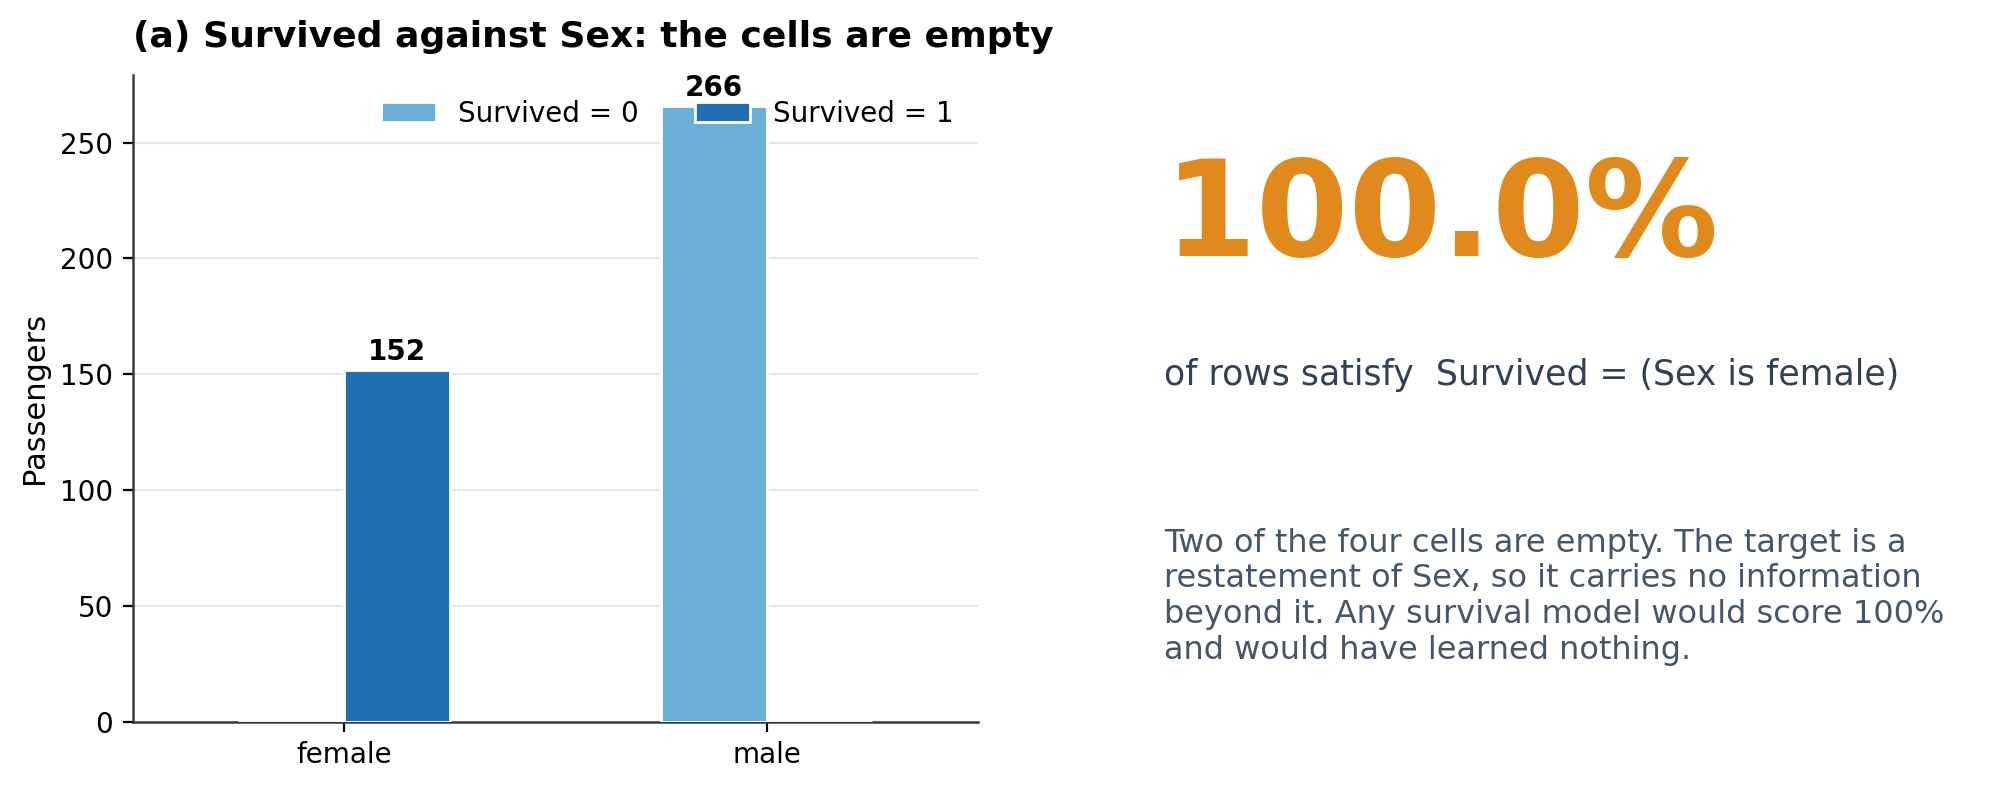
\includegraphics[width=\linewidth]{01_target_leakage.png}
\caption{The target against sex. Half the canvas is given to a single number because
that number invalidates an entire class of analysis a reader would otherwise expect.}
\end{figure}

\begin{figure}[H]\centering
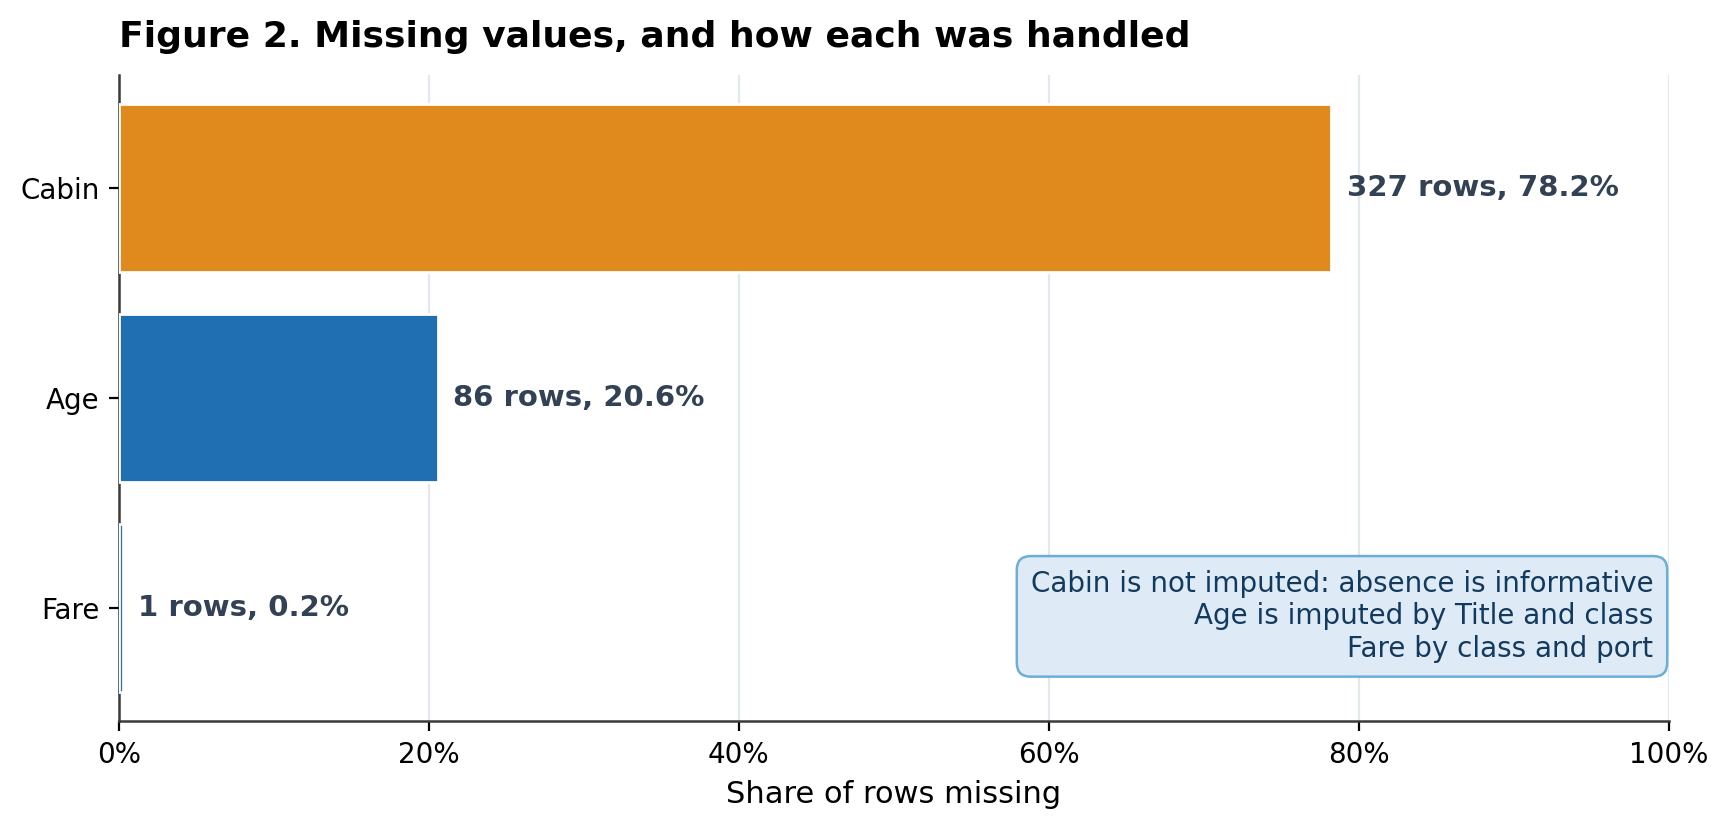
\includegraphics[width=0.94\linewidth]{02_missing_values.png}
\caption{The three incomplete columns, and the decision taken on each.}
\end{figure}

\section{Cleaning and imputation}

\begin{table}[H]\centering\caption{One decision per column, with its reason}\normalsize
\begin{tabular}{@{}lrp{7.0cm}@{}}\toprule
\textbf{Column} & \textbf{Missing} & \textbf{Decision and reason} \\ \midrule
\F{Age} & 86 &
Imputed by the median of \F{Title} and \F{Pclass} together. Title carries
life stage and class correlates with age, so the pair is far more specific than
either alone. A global median would give a three-year-old the age of an officer \\
\F{Fare} & 1 &
Imputed by the median of \F{Pclass} and \F{Embarked}, because fare is set
by class and route \\
\F{Cabin} & 327 &
\textbf{Not imputed.} Absence is informative: a number was recorded for
74.8\% of first class against 1.8\% of third.
Inventing 327 values would fabricate
78.2\% of a column \\
Zero fares & 2 rows &
\textbf{Kept.} One belongs to the chairman of the line, travelling on company
business. A zero fare is a commercial arrangement, not a recording error \\
\bottomrule\end{tabular}\end{table}

Every imputed value is flagged in \F{Age\_imputed} and \F{Fare\_imputed},
so a later reader can exclude them and see how far the conclusions move.
\textbf{No row was deleted}; twelve columns become 24.

\section{Indicators}

\begin{table}[H]\centering\caption{The manifest in seven figures}\normalsize
\begin{tabular}{@{}lr@{}}\toprule
Passengers & 418 \\
Female share & 36.4\% \\
Median age & 26.0 years \\
Median fare & 14.45 \\
Third class & 52.2\% \\
Travelled alone & 60.5\% \\
Cabin recorded & 21.8\% \\
\bottomrule\end{tabular}\end{table}

\begin{figure}[H]\centering
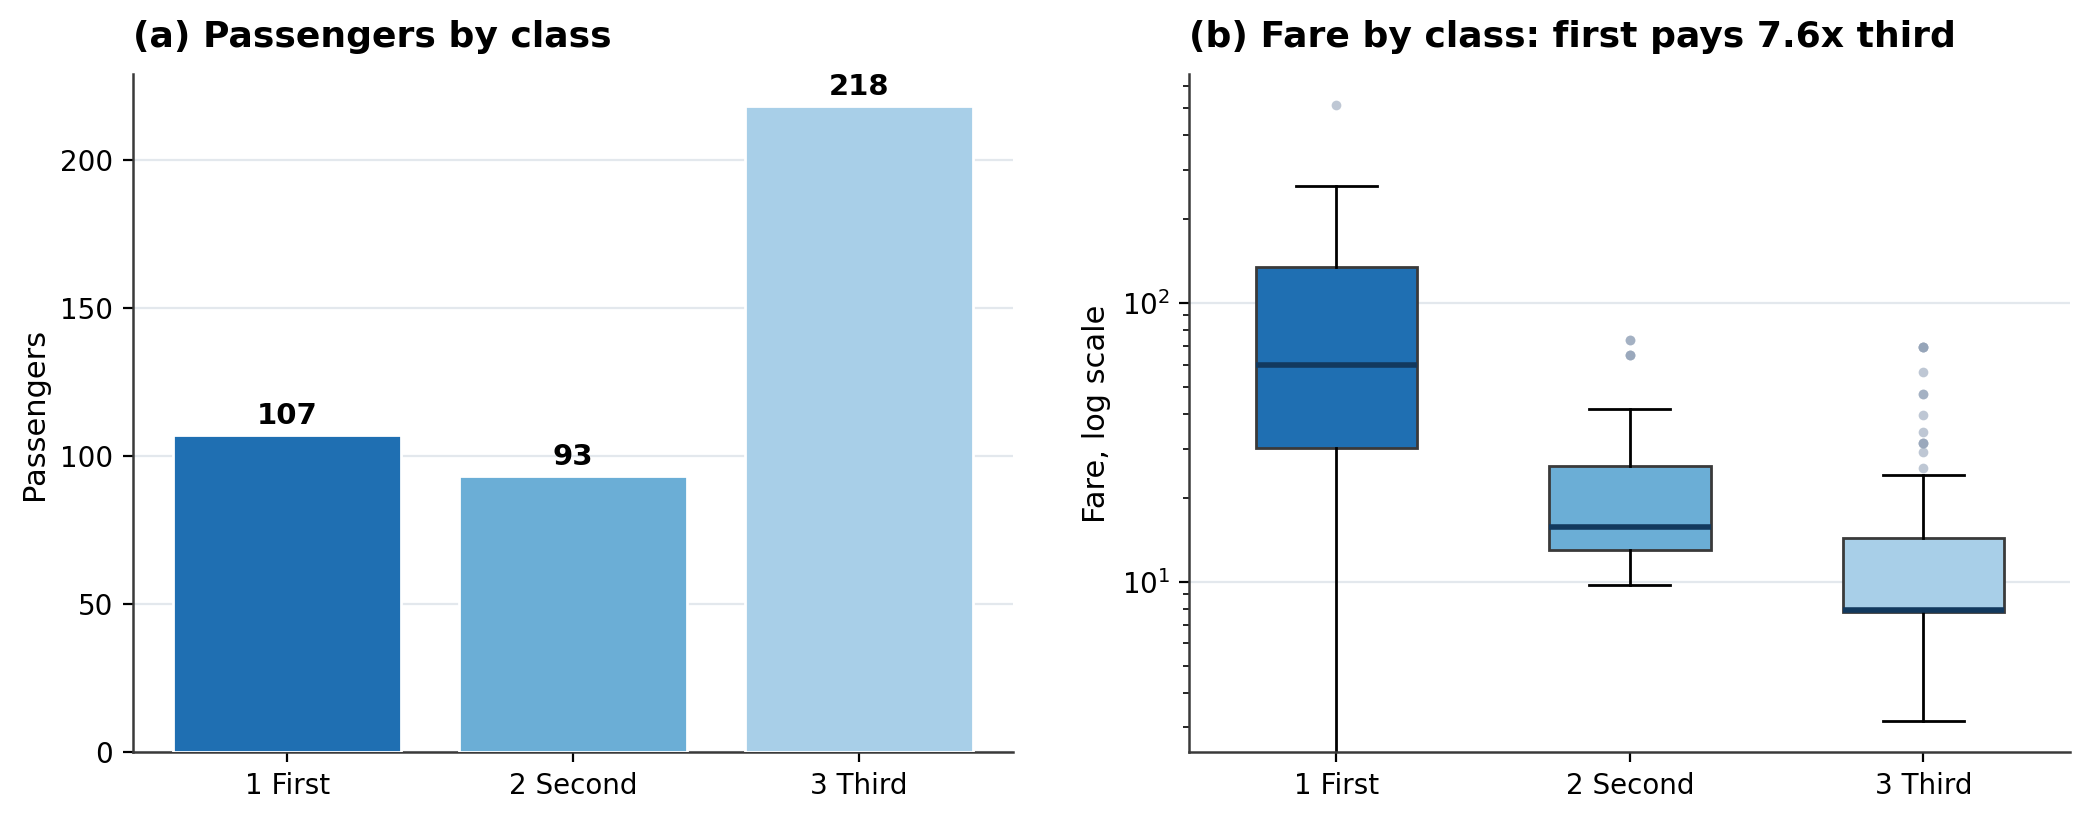
\includegraphics[width=\linewidth]{03_class_and_fare.png}
\caption{Class and fare. The box plot uses a logarithmic axis because fare spans
three orders of magnitude; a linear axis would compress every third-class ticket
into a single band.}\end{figure}

\begin{figure}[H]\centering
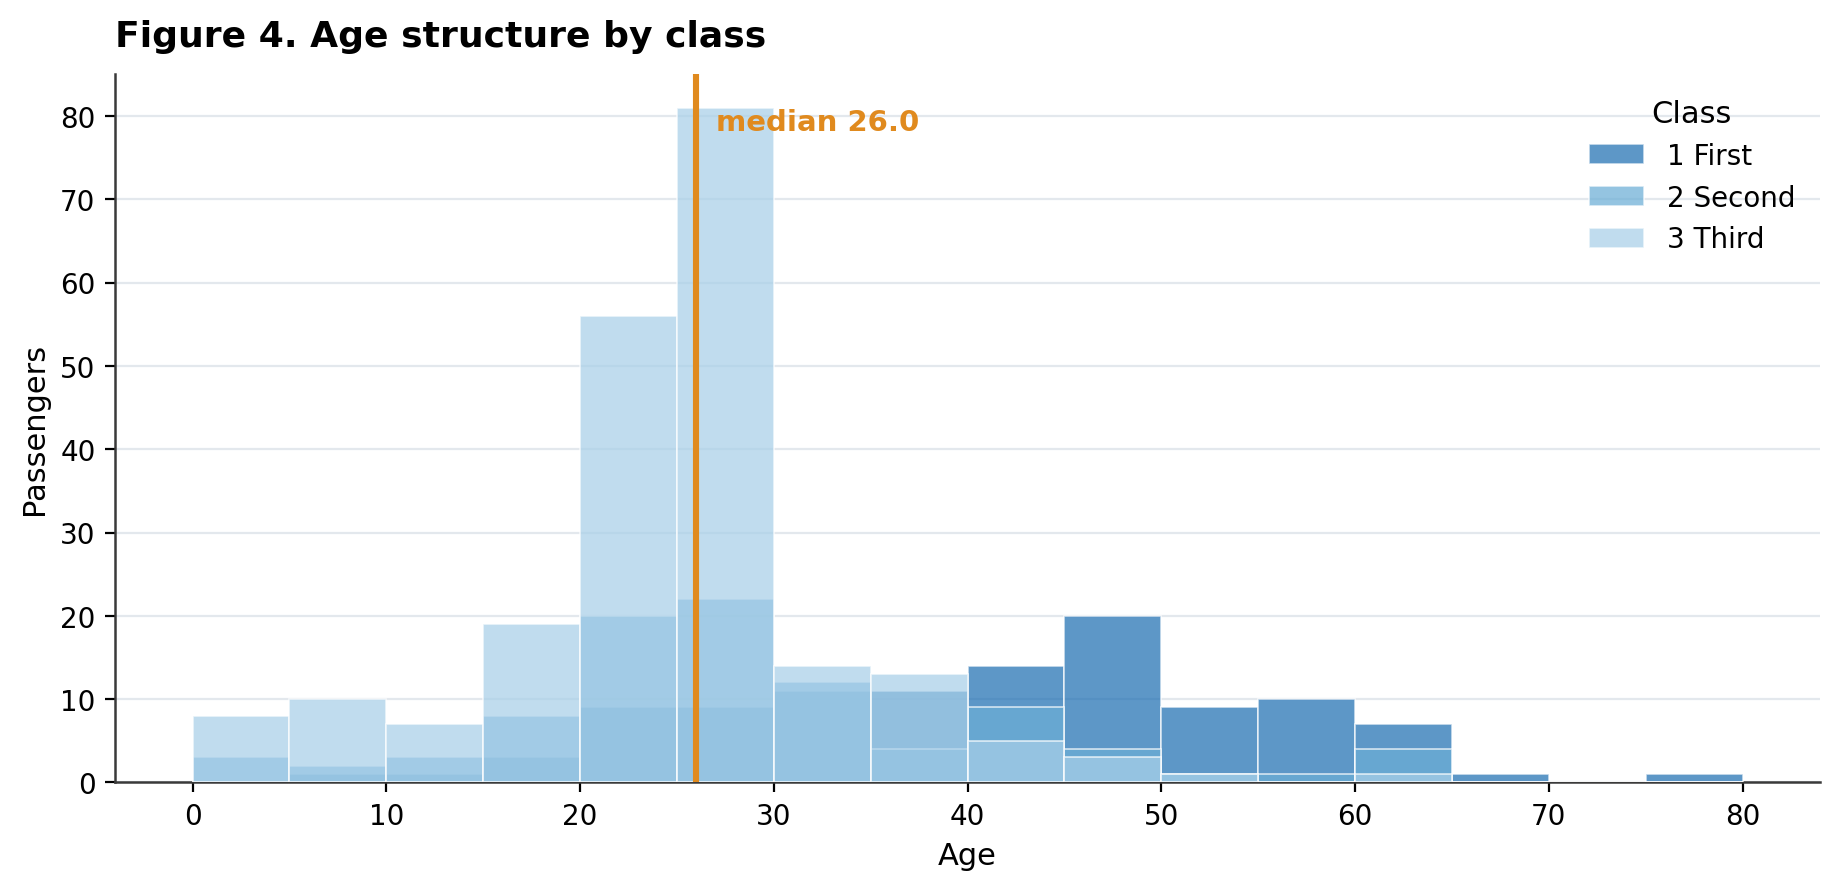
\includegraphics[width=0.94\linewidth]{04_age_structure.png}
\caption{Age structure by class, after imputation.}\end{figure}

\begin{figure}[H]\centering
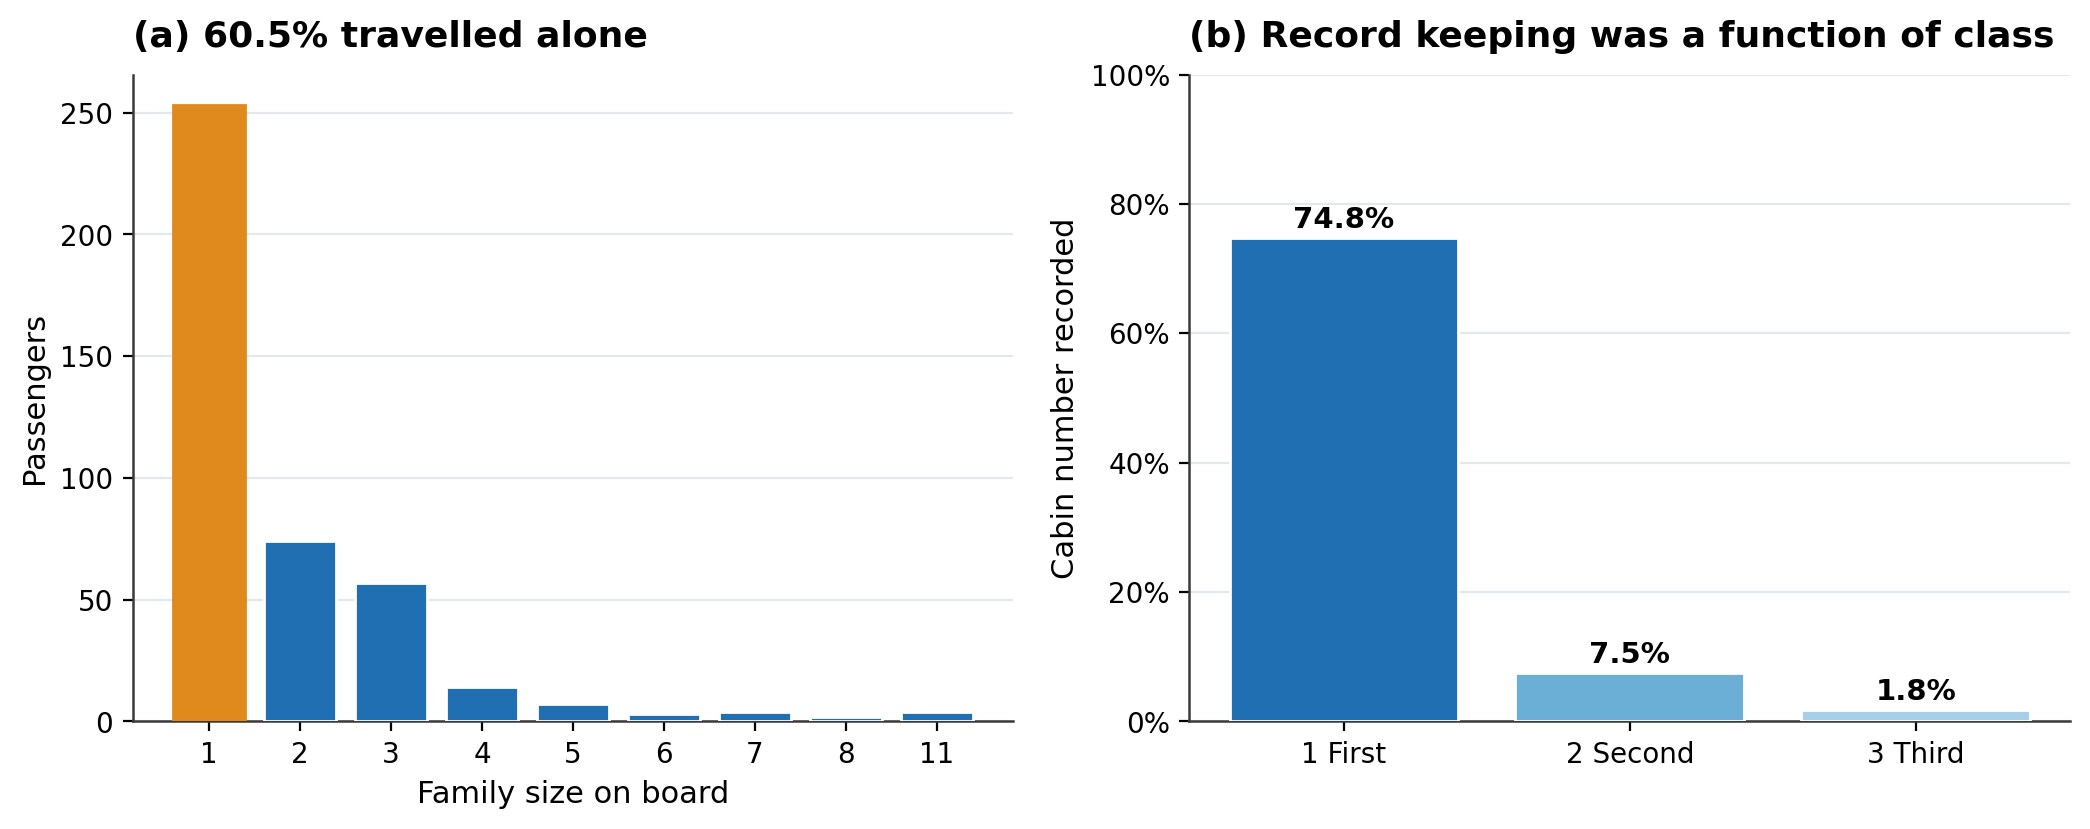
\includegraphics[width=\linewidth]{05_family_and_records.png}
\caption{Family size, and the record-keeping rate by class. Panel (b) is the evidence
behind the decision not to impute \F{Cabin}.}\end{figure}

\section{Insights and recommendations}

\subsection{The target column is unusable, and that is the headline}

\F{Survived} matches \F{Sex} on 100.0\% of rows.
Any survival analysis on this file restates the sex split.

\textbf{Recommendation.} Trace the column to its source before any modelling is
commissioned. If the labels were filled by a rule, the true ones must be recovered.
If it is an extraction error, it affects every other export from the same system.

\subsection{Three quarters of the cabin column is missing, and the gap is the signal}

The absence is not random: 74.8\% of first class against
1.8\% of third. The column measures record-keeping as much as
accommodation.

\textbf{Recommendation.} Use the derived \F{Has\_Cabin} flag as a class proxy.
Imputing \F{Cabin} would destroy the signal the gap carries.

\subsection{Fare is the clearest description of the ship}

First class paid a median fare \textbf{7.6 times} that of
third, and the range spans three orders of magnitude. Age, port and family size all
vary with class, which makes class the single most informative column.

\subsection{Most passengers travelled alone}

60.5\% had a family size of one, and only
23.2\% shared a ticket with anyone. An analysis
assuming family groups as the unit of observation would describe a minority.

\subsection{One age in five had to be reconstructed}

20.6\% of ages were imputed, from title and class rather
than a global median. Every imputed value is flagged.

\section{The interactive dashboard}

\texttt{dashboard.html} is a single self-contained file: no server, no installation.
It was built with Python, Pandas and Plotly only. \textbf{No spreadsheet and no
business-intelligence tool was used at any stage}, as the brief requires.

The interface uses a left navigation bar. Each item opens a dedicated view:
Overview, Executive Summary, Passenger Analysis, Survival Analysis, Fare Analysis,
Correlation, Data Quality, Geographic, Insights \& Recommendations, Data Explorer
and About. Key performance indicators, charts and tables are rendered client-side.

\begin{figure}[H]\centering
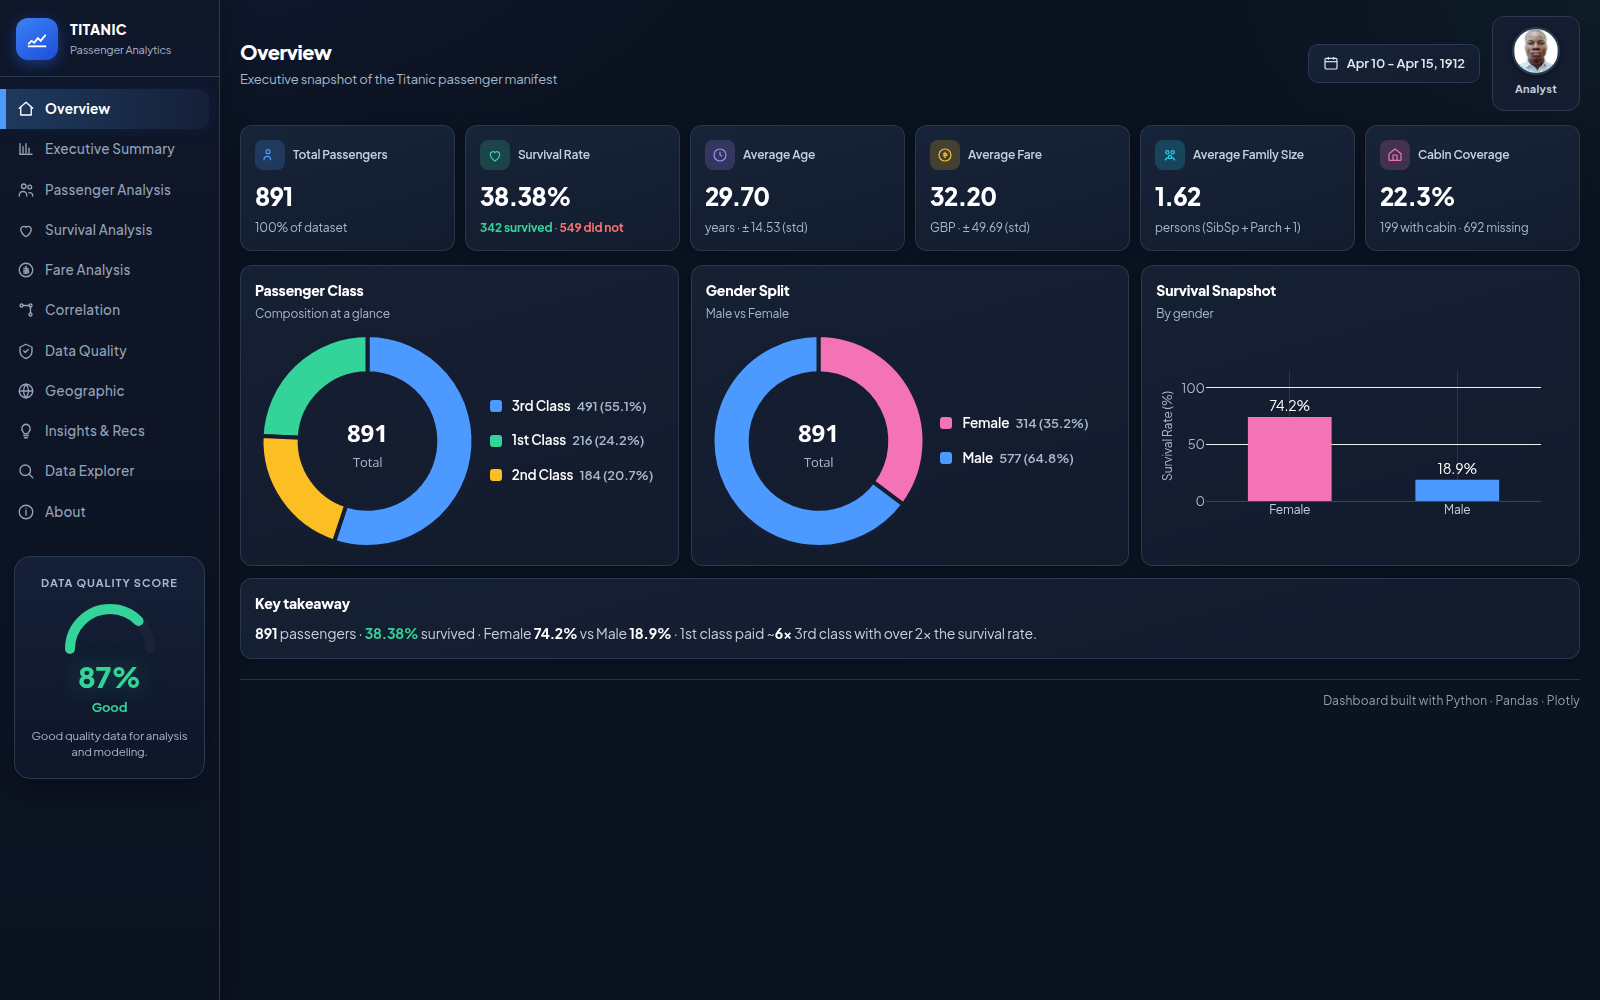
\includegraphics[width=\linewidth]{06_dashboard_overview.png}
\caption{Dashboard --- Overview. Six KPIs, composition charts and key takeaway.
Data quality score 87\% in the sidebar. Analyst photo shown in the header.}
\end{figure}

\begin{figure}[H]\centering
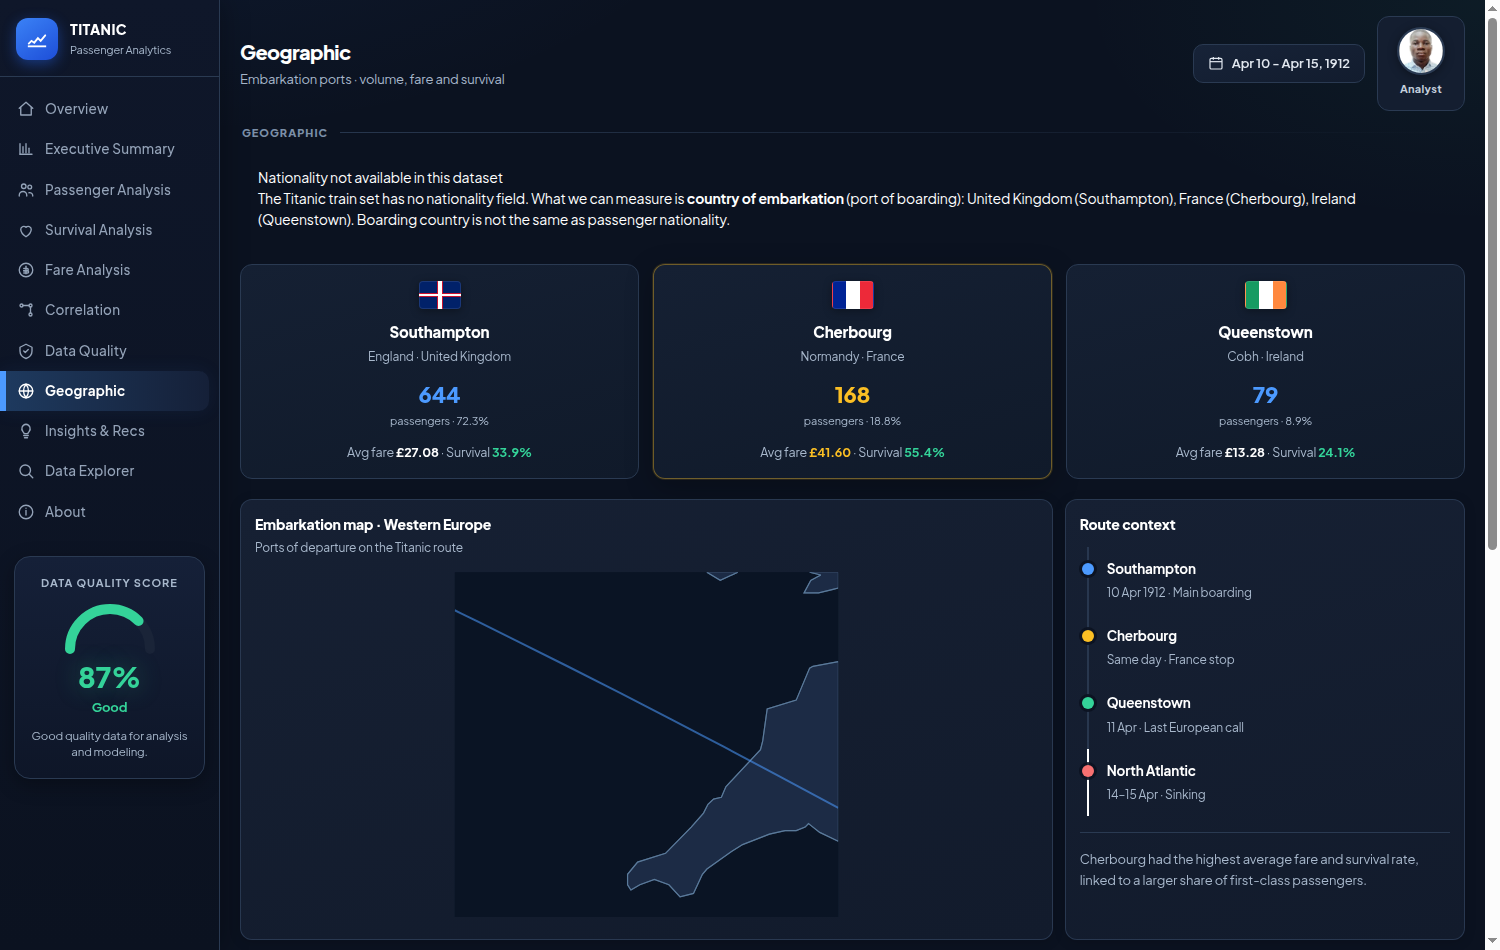
\includegraphics[width=\linewidth]{07_dashboard_geographic.png}
\caption{Dashboard --- Geographic view. Country of embarkation cards (United Kingdom,
France, Ireland), embarkation map, route timeline and port statistics.}
\end{figure}

\begin{figure}[H]\centering
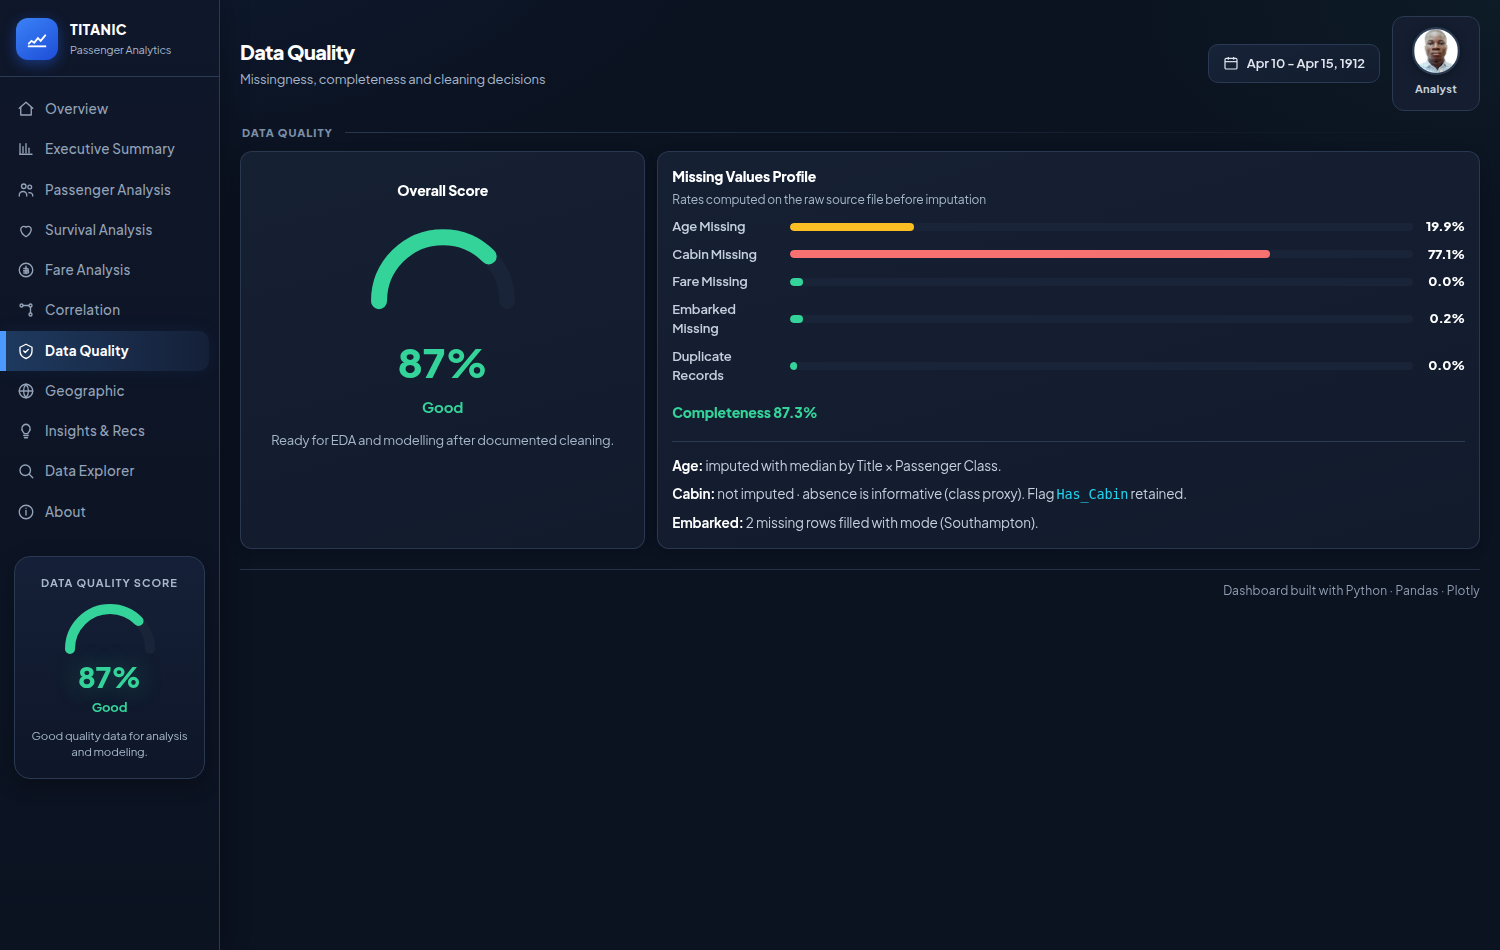
\includegraphics[width=\linewidth]{07_dashboard_quality.png}
\caption{Dashboard --- Data Quality view. Overall score, missing-value profile and
documented cleaning decisions.}
\end{figure}

\begin{figure}[H]\centering
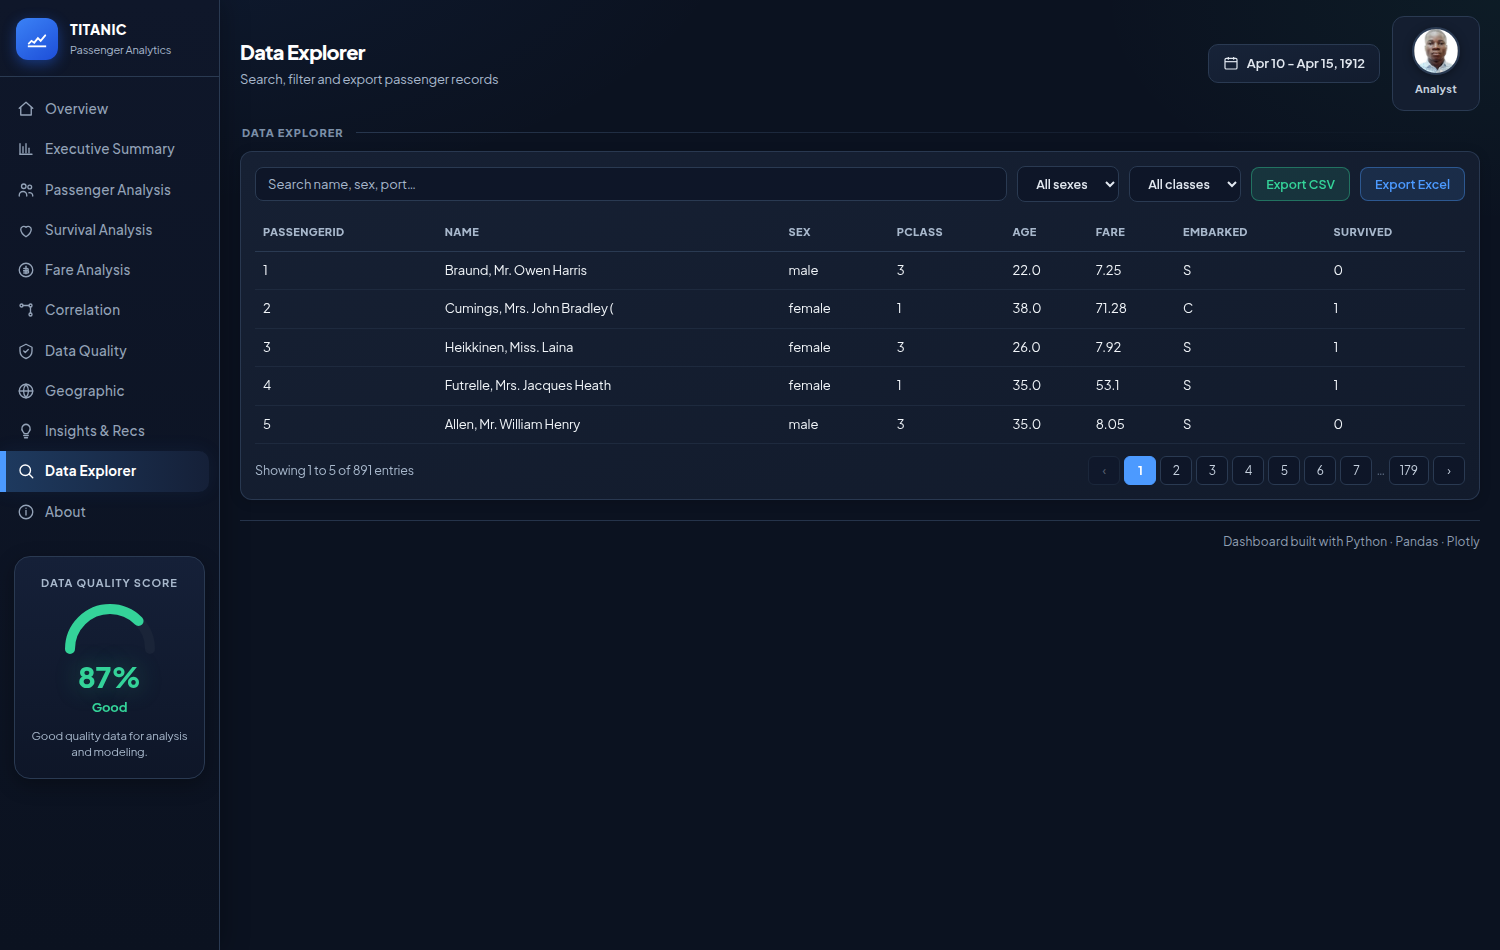
\includegraphics[width=\linewidth]{07_dashboard_explorer.png}
\caption{Dashboard --- Data Explorer. Search, filters, pagination and export of
passenger records.}
\end{figure}

\begin{figure}[H]\centering
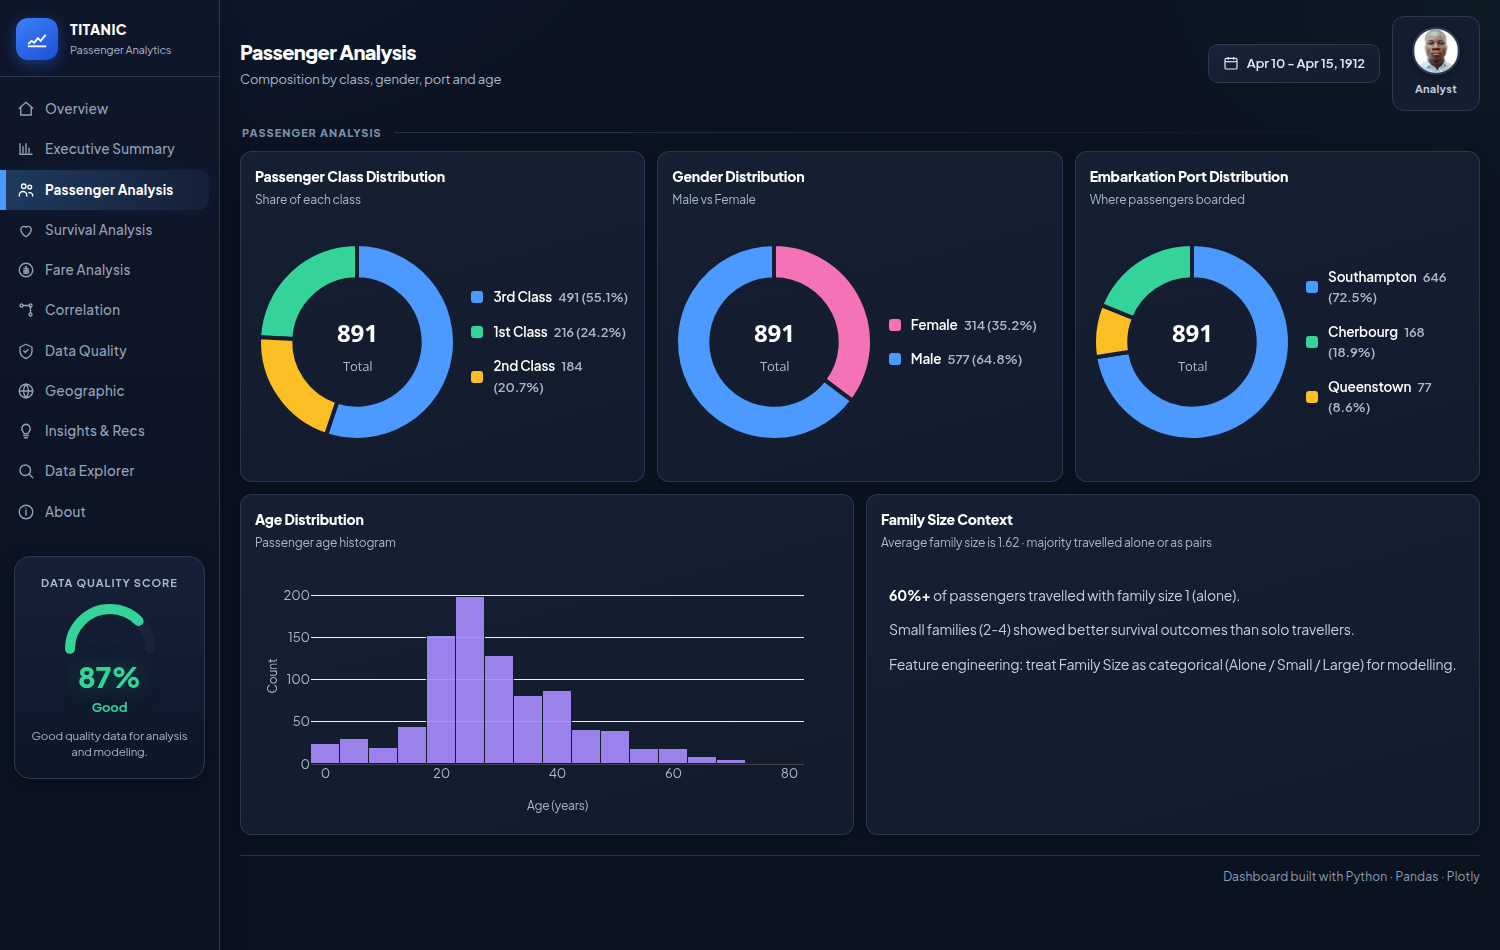
\includegraphics[width=\linewidth]{07_dashboard_passenger.png}
\caption{Dashboard --- Passenger Analysis. Class, gender and port composition with
age distribution.}
\end{figure}

\noindent\textbf{Main capabilities.}
\begin{itemize}
  \item KPI strip and executive insights on the Overview and Executive Summary views.
  \item Composition charts (class, gender, port) and survival breakdowns.
  \item Fare analysis (log-scale distribution, age--fare scatter by class).
  \item Correlation heatmap of numeric features.
  \item Data quality panel with missingness rates and cleaning decisions.
  \item Geographic view: country of embarkation (United Kingdom, France, Ireland),
        route timeline and port comparison. Nationality is \emph{not} present in the
        source file; only boarding port is measured.
  \item Data Explorer with search, filters, pagination and CSV / Excel export.
  \item Analyst photo slot in the header (optional profile image).
\end{itemize}

The cleaned table used by the dashboard is \texttt{data/manifest\_clean.csv}.
Open \texttt{dashboard.html} in a modern browser with internet access once
(so that Plotly and the typeface can load), then navigate with the sidebar.

\section{Limitations}

\textbf{The target is unusable}, as established above. Nothing in this study addresses
survival.

\textbf{418 records is a small manifest.} One title band holds a single passenger.

\textbf{One row in five carries an imputed age}, so the age distribution is smoother
than the true one.

\textbf{Fare is per ticket, not per person.} \F{FarePerPerson} is derived by
dividing by group size, but the ambiguity remains.

\textbf{Correlation, not causation.} Nothing here explains why class, age and port
covary.

\section*{Deliverables}
\addcontentsline{toc}{section}{Deliverables}

\begin{table}[H]\centering\normalsize
\begin{tabular}{@{}ll@{}}\toprule
\textbf{File} & \textbf{Content} \\ \midrule
\texttt{Passenger\_Manifest\_Analysis.ipynb} & Commented notebook, executed \\
\texttt{dashboard.html} & Interactive multi-view dashboard (Plotly) \\
\texttt{report.pdf} & The present report \\
\texttt{INSIGHTS.md} & Insights and recommendations \\
\texttt{data/manifest\_clean.csv} & Cleaned dataset, 418 rows \\
\texttt{analysis.py}, \texttt{dashboard.py} & The code, commented \\
\texttt{figures/} & Analysis figures + dashboard screenshots \\
\bottomrule\end{tabular}\end{table}

\vspace{1cm}\noindent\rule{\linewidth}{0.4pt}\\[3pt]
{\small\textbf{KOUAME Koffi Fid\`ele}\\ Data Analysis Internship\\ koffifidelek59@gmail.com}
\end{document}
